% ============================================================
%  Hands-On 1 — Pengenalan Antarmuka Sistem Operasi dan Virtual Machine
% ============================================================

\chapter{Instalasi Ubuntu pada VirtualBox}
\label{chap:handson-01}

% --- 1. Tugas ---
\section*{Tujuan dan Output Praktikum}
\subsection*{Tujuan}
    \begin{itemize}
        \item Menjelaskan langkah-langkah instalasi sistem operasi Ubuntu pada lingkungan VirtualBox.
        \item Mengonfigurasi mesin virtual sesuai dengan kebutuhan sistem (alokasi RAM, storage, dan CPU).
        \item Melakukan proses instalasi Ubuntu hingga sistem dapat dijalankan dengan baik sebagai Guest Operating System.
    \end{itemize}

\subsection*{Output}
    \begin{itemize}
        \item Mesin virtual Ubuntu yang berhasil terinstal dan dapat dijalankan pada VirtualBox.
        \item Dokumentasi proses instalasi (screenshot tahapan penting instalasi).
        \item Laporan praktikum yang memuat konfigurasi mesin virtual serta hasil verifikasi sistem.
    \end{itemize}

\section*{Alat dan Bahan}
\subsection*{Perangkat Keras}
    \begin{itemize}
        \item Laptop atau PC dengan prosesor minimal dual-core.
        \item RAM minimal 4 GB (disarankan 8 GB untuk kinerja optimal).
        \item Ruang penyimpanan kosong minimal 25 GB.
    \end{itemize}

\subsection*{Perangkat Lunak}
\begin{itemize}
    \item Sistem Operasi utama (Windows, macOS, atau Linux) sebagai Host OS.
    \item Oracle VM VirtualBox.
    \item File ISO Ubuntu.
\end{itemize}

\section*{Langkah-Langkah Praktikum}
\subsection*{Langkah-Langkah Instalasi VirtualBox}
\textit{Software yang digunakan pada praktikum kali ini adalah Oracle VM VirtualBox}
\begin{enumerate}
    \item Buka browser dan download melalui situs resmi \url{https://www.virtualbox.org/wiki/Downloads}
    \item Pilih dan klik platform Windows Hosts jika menggunakan OS windows.
    \item Lalu proses download file VirtualBox akan berjalan dan tersimpan di folder Downloads.
\end{enumerate}
\begin{figure}
    \centering
    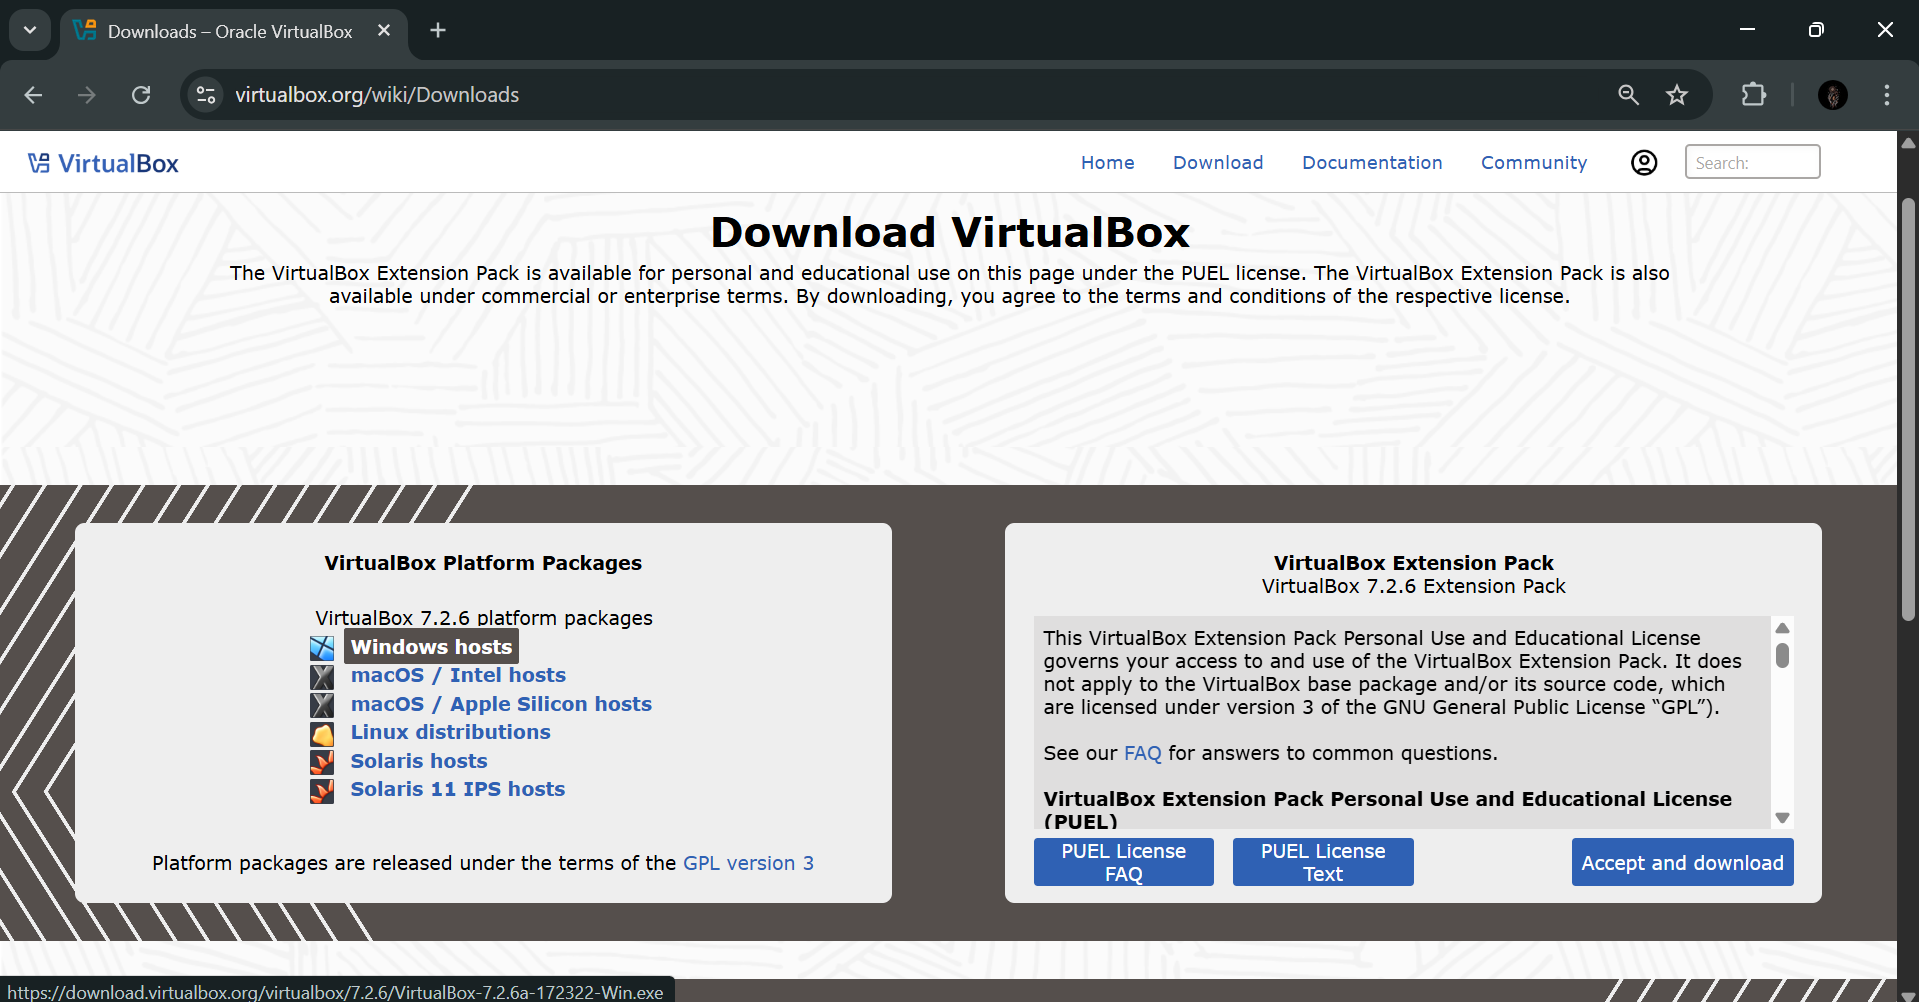
\includegraphics[width=0.5]{Figure/1/download_oracle_vm_virtualbox.png}
    \caption{Tampilan saat mendownload Oracle VM VirtualBox}
\end{figure}

% --- 2. Kesimpulan ---
\newpage
\section{Kesimpulan}

\noindent\textit{[TODO: Tuliskan kesimpulan dari praktikum yang telah dilaksanakan.
Kesimpulan hendaknya menjawab tujuan-tujuan pada modul praktikum, minimal 2--3 paragraf.]}

% --- 3. Lampiran: Bukti Penggunaan AI ---
\newpage
\section{Lampiran: Bukti Penggunaan AI}
\label{sec:h01-lampiran-ai}

Sesuai dengan kebijakan penggunaan kecerdasan buatan (AI) dalam kegiatan akademik,
praktikan \textbf{wajib} mencantumkan setiap penggunaan alat bantu AI yang dilakukan
selama pengerjaan hands-on ini. Ketidakjujuran dalam pelaporan penggunaan AI dianggap
sebagai pelanggaran integritas akademik.

\subsection{Identitas Penggunaan AI}

\begin{table}[h]
\caption{Informasi Alat AI yang Digunakan}
\label{tab:h01-ai-info}
\centering
\begin{tabulary}{\textwidth}{|L|L|}
\hline
\textbf{Keterangan}   & \textbf{Isian} \\ \hline
Nama alat AI          & \textit{(contoh: ChatGPT, GitHub Copilot, Gemini, dst.)} \\ \hline
Versi / Model         & \textit{(contoh: GPT-4o, Gemini 1.5 Pro, dst.)} \\ \hline
Tanggal penggunaan    & \textit{TODO: isi tanggal} \\ \hline
Tujuan penggunaan     & \textit{TODO: jelaskan secara singkat untuk apa AI digunakan} \\ \hline
\end{tabulary}
\end{table}

\subsection{Tangkapan Layar Percakapan AI}

Sertakan tangkapan layar (\textit{screenshot}) percakapan dengan AI sebagai
bukti otentik. Setiap gambar harus memperlihatkan \textbf{prompt} yang dikirimkan
dan \textbf{respons} yang diterima secara jelas.

\begin{figure}[h]
    \centering
    % TODO: ganti dengan screenshot percakapan AI Anda
    
\includegraphics[width=0.85\textwidth]{Figure/ifitera-header.png}
    \caption{Tangkapan Layar Percakapan AI --- Sesi 1 (TODO: ganti caption)}
    \label{fig:h01-ai-screenshot-1}
\end{figure}
